% This is samplepaper.tex, a sample chapter demonstrating the
% LLNCS macro package for Springer Computer Science proceedings;
% Version 2.20 of 2017/10/04
%
\documentclass[runningheads]{llncs}
%
\usepackage{graphicx}
\usepackage{hyperref}
% Used for displaying a sample figure. If possible, figure files should
% be included in EPS format.
%
% If you use the hyperref package, please uncomment the following line
% to display URLs in blue roman font according to Springer's eBook style:
\renewcommand\UrlFont{\color{blue}\rmfamily}
\usepackage{cite}
\usepackage{algorithm}
\usepackage{algorithmic}
\usepackage{subcaption}
\usepackage{changepage}
\usepackage{comment}
\usepackage[title]{appendix}

\begin{document}
%
\title{Improving Accuracy of Species Tree Estimation by Employing Evolutionary Multi-objective Optimization}
\author{}
\institute{}
%
\maketitle              % typeset the header of the contribution
%

\begin{abstract}
Species tree estimation from multi-locus data is complicated as biological processes can result in different loci having different evolutionary histories. Incomplete
lineage sorting (ILS), modeled by the multi-species coalescent (MSC), is considered to be a dominant cause for gene tree incongruence. Various optimization criteria (e.g., quartet consistency, pseudo-likelihood, etc.) have been shown to be statistically consistent under the MSC model, meaning that they return the true species tree with high probability given sufficiently large numbers of accurate gene trees. However, the number of genes is limited, and estimating highly accurate gene trees is difficult. Therefore, even the statistically consistent methods may fail to reconstruct highly accurate trees under practical model conditions with limited numbers of genes and in the presence of gene tree estimation error. In this study, we present a novel multi-objective optimization algorithm (NOSSGA) which combines various optimization criteria to find a suitable search space containing highly accurate species trees. Our experimental results on a collection of simulated dataset demonstrate that NOSSGA can lead us to a tree-space containing significantly better trees than ASTRAL- and MP-EST-estimated trees and their neighboring trees.

%The abstract should briefly summarize the contents of the paper in 15--250 words.

\keywords{Phylogenomics  \and Multi-objective
optimization \and Evolutionary Algorithm.}
\end{abstract} 
\section{Introduction}
In biological studies, evolutionary relationships among organisms (usually known as taxa) are inferred in the form of a phylogenetic tree. Information discovered through analyzing such a tree has benefited several branches if science including but not limited to medicine, forensics, bio-geography, epidemiology~\cite{felix2015phylogenetics}.  
\section{Problem Description}
\label{sec:problem}
We are given a set of $M$ rooted binary trees as a collection gene trees each having $N$-taxon. We need to construct the species tree, a rooted binary tree with $N$-taxon, from these gene trees by simultaneously optimizing the following three objective functions:  
\begin{enumerate}[label=$F\arabic*$.]
		
	\item Maximize QT 
	 \subitem {\footnotesize QT: number of consistent quartets (i.e., unrooted 4-taxon tree) between the species tree and the gene trees (used by ASTRAL\cite{mirarab2014astral})}
	\item Maximize TP
		\subitem {\footnotesize TP: number of consistent triplets (i.e., rooted 3-taxon tree) between the species tree and the gene trees (used by STELAR~\cite{islam2019stelar})}
	\item Maximize PL 
		\subitem {\footnotesize PL: pseudo-likelihood estimate of the species tree utilizing the underlying triplet distribution of the gene trees (used by MP-EST~\cite{mpest})}
\end{enumerate}
\textbf{In subsequent sections, we treat each objective into minimization by multiplying with -1}. Unlike traditional multi-objective optimization
problems (MOPs), here our goal is not to properly approximate the Pareto front (PF). 
%The traditional definition of convergence is may not be applicable in this problem. 
Moreover, here a dominated solution can be better in terms of tree accuracy than a non-dominated. Therefore in this paper, we try to design a special-purpose EMO algorithm which is able find a tree-space containing highly accurate species trees. 
%Each of the above functions (optimized by an existing method) has some ability to predict the species tree accuracy but none of them can necessarily lead towards the most accurate species tree. Therefore, optimizing them together, by an EMO algorithm, will generate a set of candidate solutions which is expected to contain a species tree which is more accurate than the output of the existing methods.
\section{Methodology}
\label{sec:method}
In this paper, we designed a special purpose EMO algorithm which we call as Normalized Objectives' Sum Sorting Genetic Algorithm (NOSSGA). It optimizes three objectives, with certain attentions to the nature of the problem, and generates a tree-space that contains high quality species trees. 

We encode species tree using \textit{TreeTemplate} class provided by BIO++~\cite{gueguen2013bpp} which is a collection of C++ libraries for Bioinformatics. 

We also apply NSGAII, using the same crossover, mutation and initialization method as the NOSSGA, to approximate the PF by optimizing the three objectives. 
\begin{equation}\label{eqn:nos}
NOS(x) = \sum_{i=1}^{3} \frac{F_i(x)-z_i^{min}}{z_i^{max}-z_i^{min}}
\end{equation}
where $z_i^{min}$ ($z_i^{max}$) is the minimum (maximum) value of $i^{th}$ objective $F_i$ observed so far during the search process
\subsection{Evolutionary Algorithms}
\begin{algorithm}[!htbp]
	\scriptsize
	\caption{NOSSGA}
	\textbf{Input:} $G$ (max. generations), $N$ (population size), $C_r$ (crossover rate), $M_r$ (mutation rate), $T$ (Tournament size)\\
	\textbf{Output:} $P$ (A vector of $N$ species trees)
	\begin{algorithmic}[1]\label{alg:nossga}
		\STATE{Initialize $P$ with $N$ randomly generated solutions (i.e., species trees) }
		\STATE{For each solution in $ P $, evaluate the objective functions and $NOS()$} \COMMENT{all objectives are treated as minimization, $NOS()$ defined in eqn.\ref{eqn:nos}}
		%\STATE{For each solution $x$ in $ P $, calculate NOS($x$)}
		\STATE{$g \gets 0$} \COMMENT{geenration counter}
		\WHILE{ $g < G$}
			\STATE{$Q \gets \emptyset$} \COMMENT{an empty vector that can hold $N$ solutions}
			\FOR{$i \leftarrow 1$ to $N$}	%\label{mainLoop}	
				\STATE{$S_1 \gets$ tournament\_selection($P$),} \COMMENT{based on NOS()}
				\STATE{$S_2 \gets$ random\_selection($P$)}
				\STATE{$Q[i] \gets$ mutation(crossover($S_1, S_2$))}
				%\STATE{Generate an offspring by applying crossover on $S_1, S_2$, then mutate the offspring and append the resultant solution to $Q$}		
			\ENDFOR	
			\STATE{For each solution in $ Q $, evaluate the objective functions and $NOS()$ }
			\STATE{$ R \gets P \cup Q$} \COMMENT{$R$ is a vector of $2N$ solutions}
			%\STATE{For each solution $x$ in $ R $, calculate NOS($x$)}
			\STATE{Sort the members of $ R $ in ascending order of NOS} \COMMENT{as all objectives are minimization}
			\STATE{$P \gets \emptyset$, Append $R[1]$ to $P$, Remove $R[1]$ from $R$}
			%\STATE{$P[1] \gets R[1]$}
			%\STATE{$i \gets 2$}
			\FOR{$i \leftarrow 2$ to $N$}	%\label{mainLoop}	
				\STATE{\textbf{if} $NOS$($R[1]$) $\ne$ $NOS$(Current end of $P$), \textbf{then} Append $R[1]$ to $P$ }	
				\STATE{Remove $R[1]$ from $R$}	\COMMENT{each element is shifted left by 1 position }
			\ENDFOR	
%			\FOR{$i \gets 1$ to $N$}	%\label{mainLoop}	
%				\IF{ NOS($R[i]) \ge P[i-1]$)}
%					\STATE{$P[i] \gets R[i]$}
%				\ENDIF
%				\STATE{Remove $R[i]$ from $R$}		
%			\ENDFOR	
			\STATE{For each remaining solution in $ R $, calculate the crowding distance}
			\STATE{Sort the members of $ R $  in descending order of the crowding distance}
			\STATE{Fill-up the remaining solutions for $P$ from the top of $R$}
			\STATE{$g \gets g + 1$}
		\ENDWHILE
		\STATE{\textbf{return} $P$}
	\end{algorithmic}
\end{algorithm}
\subsection{Objective Evaluation}
ASTRAL, STELAR: java code
MP-EST: Maximize branch length, c++ code
\subsection{Crossover}
PDG
\subsection{Mutation}
NNI, SPR, TBR
\subsection{Solution Initialization}
Using crossover on randomly selected pairs of gene trees.
\section{Results}
\subsection{Datasets}
%\begin{figure}
%	\centering
%	\includegraphics[width=0.6\textwidth]{Figure/10-taxon_10_replicates}
%	\caption{10-taxon.} \label{fig1}
%\end{figure}
%\begin{figure}
%	\centering
%	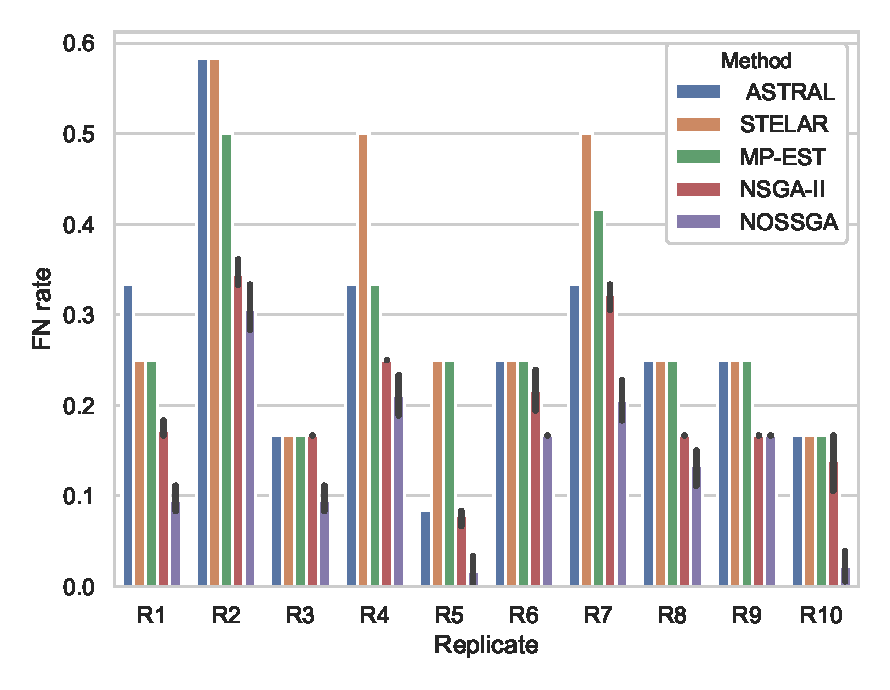
\includegraphics[width=0.6\textwidth]{Figure/15-taxon_10_replicates}
%	\caption{15-taxon.} \label{fig2}
%\end{figure}
\begin{figure}[!htbp]
	\centering
	\begin{adjustwidth}{-4.5cm}{}
	\begin{subfigure}[b]{0.5\textwidth}
		\includegraphics[width=\textwidth]{Figure/10-taxon_10_replicates}
		\caption{10-taxon}
		%\label{fig:con_pr06}
	\end{subfigure}%
	\begin{subfigure}[b]{0.5\textwidth}
		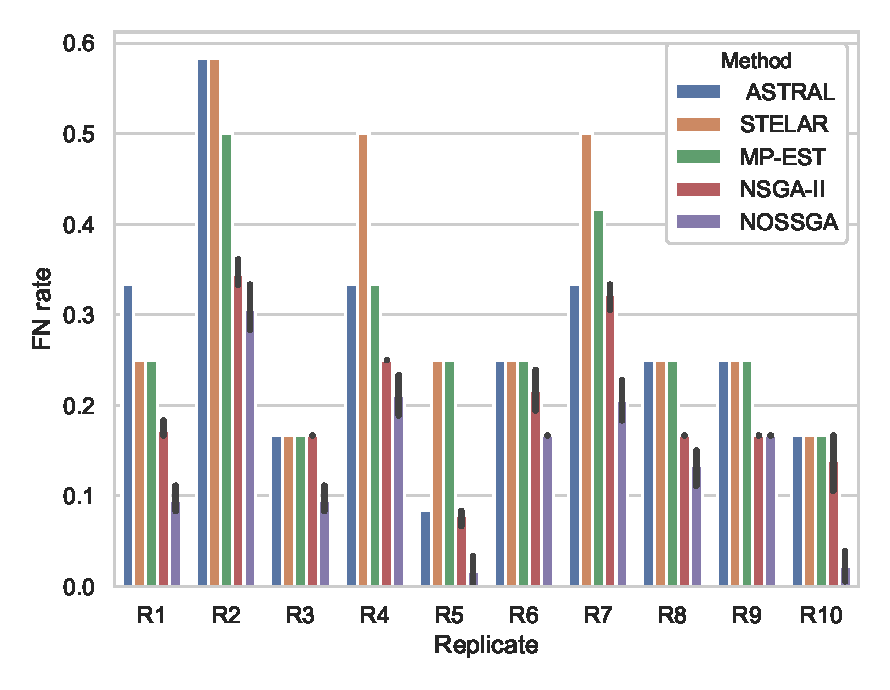
\includegraphics[width=\textwidth]{Figure/15-taxon_10_replicates}
		\caption{11-taxon}
		%\label{fig:con_pr07}
	\end{subfigure}%
	\begin{subfigure}[b]{0.5\textwidth}
		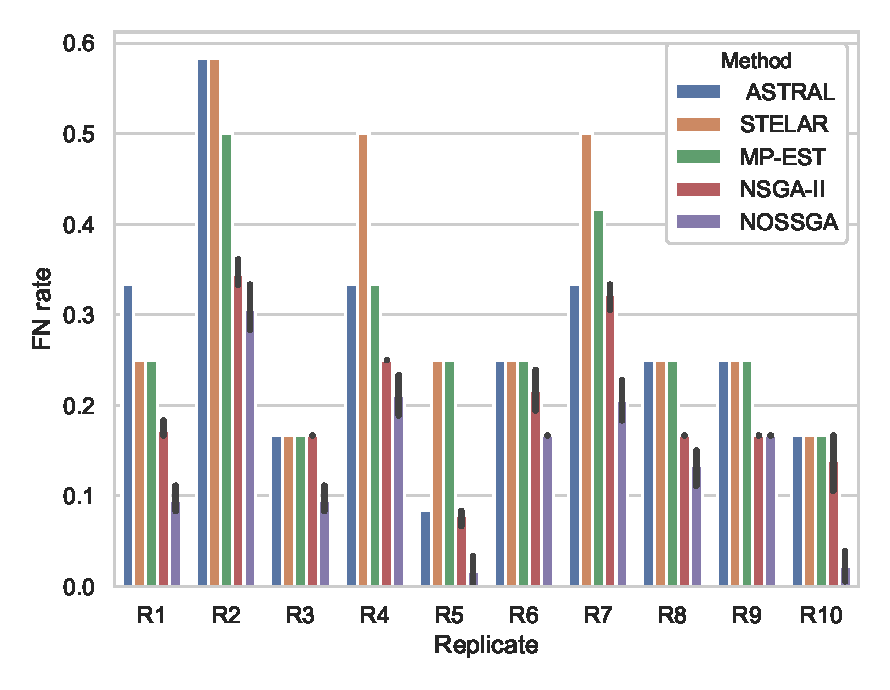
\includegraphics[width=\textwidth]{Figure/15-taxon_10_replicates}
		\caption{15-taxon}
		%\label{fig:con_pr09}
	\end{subfigure}%
	\end{adjustwidth}
	\caption{Comparison of ASTRAL, MP-EST, STELAR, NSGA-II and NOSSGA on 10 replicates of 3 datasets.}
	\label{fig:datasets}

\end{figure}
\subsection{Results on 10-taxon dataset}
\subsection{Results on 11-taxon dataset}
\subsection{Results on 15-taxon dataset}
\subsection{Discussion}
\section{Conclusion}
In this paper we introduced the problem of estimating species tree from a set of gene trees as a MOP. We showed with examples that the existing method, optimizing a single criterion, may overshoot the criterion and thus deviate from the true species tree. We selected three objectives from three existing methods. Unlike traditional MOPs, in this problem a dominated solution is often important than a non-dominated one and hence we cannot rely on the PF to contain better solutions. Therefore, we designed a specialized EMO algorithm, namely, NOSSGA, in which we embed particular traits to be able to return a tree-space containing highly accurate trees. We analyzed the difference of behavior between NOSSGA and the popular NSGAII. Finally, we found the accuracy of the best trees offered by NOSSGA is quite better three existing methods. We are currently working to find our a way to filter a limited number of better trees from the final population without the knowledge of true tree provided with the simulated dataset. Furthermore, we are improving the efficiency of NOSSGA to make it scalable for larger datasets. 



%
% ---- Bibliography ----
%
% BibTeX users should specify bibliography style 'splncs04'.
% References will then be sorted and formatted in the correct style.
%
\bibliographystyle{splncs04}
\bibliography{main_bib}

%\begin{subappendices}
\renewcommand{\thesection}{\Alph{section}}%
% or try \arabic{section}

\section{Also you should know this}
Really.
\section{And I also came across this}
But I need to put this in an appendix so that my paper is not too long.
\end{subappendices}
\end{document}
